Phần phép tính quan trọng tiếp theo sau khi đã tìm được các biểu diễn số nguyên lớn là cài đặt phép toán modulo. Nếu dùng kiểu dữ liệu \textbf{number\_t} 
như phần trước trình bày thì phần này không có gì đặc biệt vì chỉ cần dùng phép toán $\%$ của kiểu dữ liệu. Nếu cài đặt lại kiểu dữ liệu số nguyên lớn thì phần này cực kì quan trọng vì tất cả các bước xử lý trong các bước tiếp theo đều dùng tới phép modulo.

Thực nghiệm cho thấy cách tính modulo truyền thống như \textit{Thuật toán \ref{alg:mod}} khi tính cho số nguyên lớn rất chậm, 
đồ án đã cài đặt thuật toán modulo theo bài báo \cite{Will14computingmod}, nội dung của thuật toán này thể hiện trong  \textit{Hình \ref{fig:modwithoutmod}}.

Với việc cài đặt thuật tóan modulo cải tiến, tốc độ chương trình được cải thiện rất nhiều.
\newpage
\begin{algorithm}
\caption{Thuật toán modulo}\label{alg:mod}
\hspace*{\algorithmicindent} \textbf{Input:} BigInt a, BigInt b\\
\hspace*{\algorithmicindent} \textbf{Output:} a \% b
\begin{algorithmic}[1]
\Procedure{Mod}{$a,b$}
\While{$a > b$}
\State $a\gets a - b$
\EndWhile\label{euclidendwhile}
\State \textbf{return} $a = b $ ? 0 : $a$
\EndProcedure
\end{algorithmic}
\end{algorithm}

\begin{figure}[!h]
    \centering
    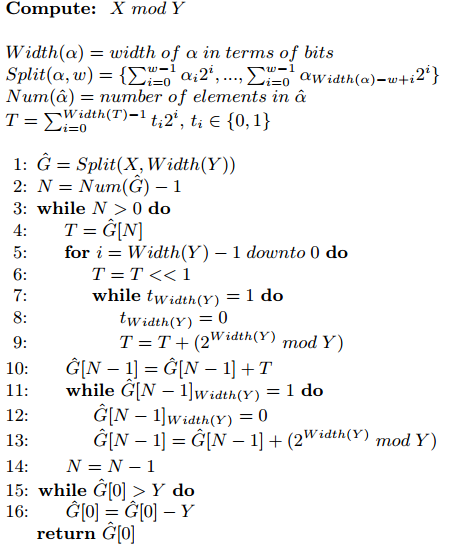
\includegraphics[width=1\textwidth]{image/mod_without_mod.PNG}
	\centering
	\caption{\label{fig:modwithoutmod} Thuật toán tính nhanh Mod trong \cite{Will14computingmod}}
\end{figure}


